\documentclass[12pt,a4paper]{article}

% ── Packages ──────────────────────────────────────────────────────────────────
\usepackage[top=2.5cm, bottom=2.5cm, left=2.5cm, right=2.5cm]{geometry}
\usepackage{tikz}
\usetikzlibrary{shapes.geometric, arrows.meta, positioning, fit, backgrounds, calc}
\usepackage{xcolor}
\usepackage{booktabs}
\usepackage{tabularx}
\usepackage{array}
\usepackage{longtable}
\usepackage{hyperref}
\usepackage{enumitem}
\usepackage{titlesec}
\usepackage{fancyhdr}
\usepackage{parskip}
\usepackage[T1]{fontenc}
\usepackage{amssymb}
\usepackage{listings}
\usepackage{caption}
\usepackage{float}
\usepackage{graphicx}
\usepackage{multicol}

% ── Colours ──────────────────────────────────────────────────────────────────
\definecolor{clientblue}{RGB}{210,228,255}
\definecolor{gatewaygreen}{RGB}{210,240,220}
\definecolor{svcyellow}{RGB}{255,249,210}
\definecolor{dbgray}{RGB}{225,225,225}
\definecolor{mqorange}{RGB}{255,232,210}
\definecolor{redisred}{RGB}{255,218,218}
\definecolor{bordercolor}{RGB}{80,80,80}
\definecolor{lightgray}{RGB}{245,245,245}
\definecolor{tablegray}{RGB}{240,240,240}

% ── Section styling ─────────────────────────────────────────────────────────
\titleformat{\section}{\large\bfseries\color{black}}{{\thesection}}{1em}{}[\titlerule]
\titleformat{\subsection}{\normalsize\bfseries\color{black}}{{\thesubsection}}{1em}{}

% ── Header / Footer ─────────────────────────────────────────────────────────
\pagestyle{fancy}
\fancyhf{}
\lhead{\small\textbf{Journey Booking System --- Final Report}}
\rhead{\small CS7NS6 --- Exercise 2}
\cfoot{\thepage}
\renewcommand{\headrulewidth}{0.4pt}

% ── Hyperref ─────────────────────────────────────────────────────────────────
\hypersetup{
  colorlinks=true,
  linkcolor=black,
  urlcolor=black,
  citecolor=black,
  pdftitle={Journey Booking System — Final Report},
}

% ── Table helpers ────────────────────────────────────────────────────────────
\newcolumntype{L}[1]{>{\raggedright\arraybackslash}p{#1}}
\newcolumntype{C}[1]{>{\centering\arraybackslash}p{#1}}

% ── Code listing style ───────────────────────────────────────────────────────
\lstset{
  basicstyle=\ttfamily\small,
  breaklines=true,
  frame=single,
  framerule=0.4pt,
  rulecolor=\color{black},
  backgroundcolor=\color{lightgray},
  xleftmargin=1em,
  framexleftmargin=0.5em,
}

% ── TikZ styles ──────────────────────────────────────────────────────────────
\tikzset{
  base/.style={draw=bordercolor, line width=0.8pt, align=center,
               font=\small, minimum height=1cm},
  client/.style   = {base, rounded corners=6pt, fill=clientblue,  minimum width=3.2cm},
  gateway/.style  = {base, rounded corners=6pt, fill=gatewaygreen, minimum width=6cm, minimum height=1.5cm},
  service/.style  = {base, rounded corners=4pt, fill=svcyellow,   minimum width=2.4cm},
  database/.style = {base, cylinder, shape border rotate=90, aspect=0.3,
                     fill=dbgray, minimum width=1.8cm, minimum height=1cm},
  broker/.style   = {base, rounded corners=4pt, fill=mqorange,    minimum width=2.6cm},
  cache/.style    = {base, cylinder, shape border rotate=90, aspect=0.3,
                     fill=redisred, minimum width=1.8cm, minimum height=1cm},
  consumer/.style = {base, rounded corners=4pt, fill=svcyellow,   minimum width=3.2cm, minimum height=1.1cm},
  arr/.style      = {-{Stealth[length=5pt]}, line width=0.8pt, color=bordercolor},
  darr/.style     = {-{Stealth[length=5pt]}, line width=0.7pt, dashed, color=bordercolor},
}

% ─────────────────────────────────────────────────────────────────────────────
\begin{document}

% ── Title Page ───────────────────────────────────────────────────────────────
\begin{titlepage}
  \centering
  \vspace*{2cm}
  {\LARGE\bfseries Journey Booking System\par}
  \vspace{0.4cm}
  {\Large Final Report\par}
  \vspace{1.5cm}
  \rule{0.6\textwidth}{0.4pt}\par
  \vspace{0.8cm}
  {\large\textbf{Module:} CS7NS6 Distributed Systems --- Exercise 2\par}
  \vspace{0.3cm}
  {\large\textbf{Group:} J\par}
  \vspace{0.3cm}
  {\large\textbf{Date:} \today\par}
  \vspace{2cm}

  \begin{tabular}{l l l}
    \toprule
    \textbf{Name} & \textbf{Service Responsibility} & \textbf{Signature} \\
    \midrule
    Parth Deshmukh        & User Service                  & \rule{3cm}{0.4pt} \\[0.4cm]
    Tanmay Ghosh          & Journey Service               & \rule{3cm}{0.4pt} \\[0.4cm]
    Sneha Meto            & Conflict Detection Service    & \rule{3cm}{0.4pt} \\[0.4cm]
    Aditya Kumar Singh    & Notification Service          & \rule{3cm}{0.4pt} \\[0.4cm]
    Saurabh Deshmukh      & Enforcement Service           & \rule{3cm}{0.4pt} \\[0.4cm]
    Sai Eeshwar Divaakar  & Analytics \& Monitoring Service & \rule{3cm}{0.4pt} \\[0.4cm]
    \bottomrule
  \end{tabular}
\end{titlepage}

% ── Table of Contents ────────────────────────────────────────────────────────
\tableofcontents
\newpage

% ═════════════════════════════════════════════════════════════════════════════
\section{Requirements}
% ═════════════════════════════════════════════════════════════════════════════

\subsection{System Overview}

The Journey Booking System is a globally-accessible, fault-tolerant distributed system that enables road-vehicle drivers to pre-book journeys before travelling. No driver may begin a journey without a confirmed booking. The system checks for scheduling conflicts on road segments, notifies drivers in real time, and allows roadside enforcement agents to verify active bookings.

\subsection{Functional Requirements}

\begin{table}[H]
\centering
\small
\caption{Functional Requirements}
\begin{tabularx}{\textwidth}{C{0.6cm} L{3.5cm} X}
  \toprule
  \textbf{ID} & \textbf{Requirement} & \textbf{Description} \\
  \midrule
  F1 & User Registration \& Authentication & Drivers and enforcement agents register with credentials. JWT-based authentication grants access tokens for subsequent API calls. \\
  F2 & Vehicle Registration & Drivers register one or more vehicles (registration plate) against their account. \\
  F3 & Journey Booking & Drivers request a journey by specifying origin, destination, departure time, and vehicle. The system validates the request and checks for road-capacity conflicts. \\
  F4 & Conflict Detection & The system prevents over-allocation of road segments by modelling roads as geographic grid cells and enforcing per-cell capacity limits in serialisable transactions. \\
  F5 & Multi-Region Booking & Journeys spanning multiple regions (e.g.\ Republic of Ireland and Northern Ireland) are coordinated via a two-phase hold/commit saga across regional conflict services. \\
  F6 & Journey Cancellation & Drivers can cancel confirmed bookings; capacity is released and all downstream services are notified via events. \\
  F7 & Real-Time Notifications & Drivers receive WebSocket push notifications for booking confirmation, rejection, start, and completion events. \\
  F8 & Enforcement Verification & Roadside agents verify active bookings by vehicle registration plate or driver licence number. Results are returned from a Redis cache for low-latency lookups. \\
  F9 & Analytics \& Monitoring & All journey lifecycle events are logged. Hourly aggregations, service health dashboards, and Postgres replica-lag metrics are exposed via API. \\
  F10 & Idempotent Booking & Duplicate booking requests (same idempotency key) return the cached result rather than creating a second journey. \\
  \bottomrule
\end{tabularx}
\end{table}

\subsection{Non-Functional Requirements}

\begin{table}[H]
\centering
\small
\caption{Non-Functional Requirements}
\begin{tabularx}{\textwidth}{C{0.6cm} L{3.5cm} X}
  \toprule
  \textbf{ID} & \textbf{Requirement} & \textbf{Description} \\
  \midrule
  NF1 & Fault Tolerance & The system must continue operating (possibly in degraded mode) when individual services, databases, or message brokers fail. \\
  NF2 & Partition Tolerance & Network partitions are detected automatically; affected services flag responses as stale and queue writes for replay on merge. \\
  NF3 & At-Least-Once Delivery & Events are delivered to all consumers at least once via a transactional outbox and consumer-side deduplication. \\
  NF4 & Data Durability & All databases use streaming replication (primary + replica). Redis uses Sentinel with a 3-node quorum for automatic failover. \\
  NF5 & Low-Latency Enforcement & Enforcement lookups are served from Redis cache, falling back to the Journey Service API only on cache miss. \\
  NF6 & Rate Limiting & The API gateway enforces three rate-limiting zones: authentication (5~req/s), booking (10~req/s), and general (30~req/s). \\
  NF7 & Scalability & Stateless services behind HAProxy + nginx allow horizontal scaling. Each service owns its database, avoiding shared-state bottlenecks. \\
  NF8 & Observability & Correlation IDs (\texttt{X-Request-ID}) propagate across all services. Partition status, replica lag, and aggregated health are exposed via dedicated endpoints. \\
  \bottomrule
\end{tabularx}
\end{table}

\subsection{Requirements Not Fully Addressed}

\begin{itemize}[nosep]
  \item \textbf{Compensating transactions}: The saga rejects bookings on conflict-service failure but does not retry or compensate.
  \item \textbf{Distributed tracing visualisation}: Correlation IDs propagate across services but no span visualisation (e.g.\ Jaeger) is integrated.
  \item \textbf{Cache warming}: The enforcement cache starts cold on service restart; no pre-population mechanism is implemented.
  \item \textbf{Token blacklisting}: Logout does not invalidate JWT tokens server-side.
\end{itemize}

% ═════════════════════════════════════════════════════════════════════════════
\section{Specification}
% ═════════════════════════════════════════════════════════════════════════════

The system is composed of six microservices, an API gateway layer, and shared infrastructure (PostgreSQL, Redis, RabbitMQ). This section specifies each service's API and fault-mode behaviour.

\subsection{Service APIs}

\subsubsection{User Service (Python, port 8001)}

\begin{table}[H]
\centering\small
\begin{tabularx}{\textwidth}{l l X}
  \toprule
  \textbf{Method} & \textbf{Endpoint} & \textbf{Description} \\
  \midrule
  POST & \texttt{/api/users/register}        & Register a driver account \\
  POST & \texttt{/api/users/register/agent}   & Register an enforcement agent \\
  POST & \texttt{/api/users/login}            & Authenticate; returns JWT \\
  GET  & \texttt{/api/users/profile}          & Retrieve own profile (auth) \\
  GET  & \texttt{/api/users/license/\{num\}}  & Look up user by licence number \\
  POST & \texttt{/api/users/vehicles}         & Register a vehicle (auth) \\
  GET  & \texttt{/api/users/vehicles}         & List own vehicles (auth) \\
  \bottomrule
\end{tabularx}
\end{table}

\subsubsection{Journey Service (Python, port 8002)}

\begin{table}[H]
\centering\small
\begin{tabularx}{\textwidth}{l l X}
  \toprule
  \textbf{Method} & \textbf{Endpoint} & \textbf{Description} \\
  \midrule
  POST   & \texttt{/api/journeys/}                     & Book a journey (idempotency key header) \\
  GET    & \texttt{/api/journeys/}                      & List own journeys (paginated) \\
  GET    & \texttt{/api/journeys/\{id\}}                & Get journey details \\
  DELETE & \texttt{/api/journeys/\{id\}}                & Cancel a journey \\
  GET    & \texttt{/api/journeys/vehicle/\{reg\}/active} & Active journeys for a vehicle \\
  GET    & \texttt{/api/journeys/user/\{uid\}/active}   & Active journeys for a user \\
  GET    & \texttt{/health/partitions}                  & Partition state of all dependencies \\
  POST   & \texttt{/admin/recovery/drain-outbox}        & Force-drain the transactional outbox \\
  \bottomrule
\end{tabularx}
\end{table}

\subsubsection{Conflict Service (Go, ports 8003/8007)}

Two instances run: one for the Republic of Ireland (IE) and one for Northern Ireland (NI).

\begin{table}[H]
\centering\small
\begin{tabularx}{\textwidth}{l l X}
  \toprule
  \textbf{Method} & \textbf{Endpoint} & \textbf{Description} \\
  \midrule
  POST & \texttt{/api/conflicts/check}              & Atomic capacity check \& reserve \\
  POST & \texttt{/api/conflicts/hold}               & Phase-1 hold (multi-region saga) \\
  POST & \texttt{/api/conflicts/commit/\{id\}}      & Phase-2 commit \\
  POST & \texttt{/api/conflicts/rollback/\{id\}}    & Phase-2 rollback \\
  POST & \texttt{/api/conflicts/cancel/\{jid\}}     & Release capacity on cancellation \\
  GET  & \texttt{/api/routes}                       & List predefined routes with waypoints \\
  GET  & \texttt{/api/region/info}                  & Regional metadata \\
  POST & \texttt{/api/simulate/\{action\}}          & Inject faults for testing \\
  \bottomrule
\end{tabularx}
\end{table}

\subsubsection{Notification Service (Go, port 8004)}

\begin{table}[H]
\centering\small
\begin{tabularx}{\textwidth}{l l X}
  \toprule
  \textbf{Method} & \textbf{Endpoint} & \textbf{Description} \\
  \midrule
  GET & \texttt{/api/notifications/}       & Retrieve past notifications (max 50) \\
  WS  & \texttt{/ws/notifications/\{token\}} & WebSocket push channel \\
  \bottomrule
\end{tabularx}
\end{table}

\subsubsection{Enforcement Service (Python, port 8005)}

\begin{table}[H]
\centering\small
\begin{tabularx}{\textwidth}{l l X}
  \toprule
  \textbf{Method} & \textbf{Endpoint} & \textbf{Description} \\
  \midrule
  GET & \texttt{/api/enforcement/verify/vehicle/\{plate\}}  & Verify by registration plate \\
  GET & \texttt{/api/enforcement/verify/license/\{num\}}    & Verify by licence (24h cache) \\
  GET & \texttt{/health/partitions}                         & Partition detection state \\
  \bottomrule
\end{tabularx}
\end{table}

\subsubsection{Analytics Service (Go, port 8006)}

\begin{table}[H]
\centering\small
\begin{tabularx}{\textwidth}{l l X}
  \toprule
  \textbf{Method} & \textbf{Endpoint} & \textbf{Description} \\
  \midrule
  GET & \texttt{/api/analytics/stats}            & Real-time statistics \\
  GET & \texttt{/api/analytics/hourly}           & Hourly aggregated statistics \\
  GET & \texttt{/api/analytics/events}           & Filterable event log \\
  GET & \texttt{/api/analytics/replica-lag}      & Postgres streaming replication lag \\
  GET & \texttt{/api/analytics/health/services}  & Aggregated health of all services \\
  \bottomrule
\end{tabularx}
\end{table}

\subsection{Asynchronous Event Bus}

All inter-service asynchronous communication uses a RabbitMQ topic exchange (\texttt{journey\_events}). The following routing keys are used:

\begin{table}[H]
\centering\small
\begin{tabularx}{\textwidth}{l X}
  \toprule
  \textbf{Routing Key} & \textbf{Consumers} \\
  \midrule
  \texttt{journey.confirmed} & Notification, Analytics, Enforcement, Conflict (NI) \\
  \texttt{journey.rejected}  & Notification, Analytics \\
  \texttt{journey.cancelled} & Notification, Analytics, Conflict (capacity release) \\
  \texttt{journey.started}   & Notification, Analytics \\
  \texttt{journey.completed} & Notification, Analytics \\
  \texttt{user.registered}   & Analytics \\
  \bottomrule
\end{tabularx}
\end{table}

\subsection{Behaviour Under Faults}

\begin{table}[H]
\centering\small
\caption{Fault-mode behaviour}
\begin{tabularx}{\textwidth}{L{3cm} X}
  \toprule
  \textbf{Fault} & \textbf{System Behaviour} \\
  \midrule
  RabbitMQ down & Journey is created and confirmed in the database. The outbox event is written transactionally. When RabbitMQ recovers, the background outbox publisher drains queued events. Downstream consumers receive events with at-least-once semantics. \\
  \addlinespace
  Conflict Service down & The circuit breaker in the Journey Service opens after 3 consecutive failures (30s timeout). Subsequent booking requests fail fast with a clear error rather than timing out. On recovery, the circuit half-opens and probes before closing. \\
  \addlinespace
  Redis failover & Redis Sentinel (quorum of 3) automatically promotes the replica. All services reconnect to the new primary via Sentinel discovery. Brief interruption in cache reads during promotion. \\
  \addlinespace
  Postgres replica down & Services fall back to reading from the primary. The \texttt{replica-lag} endpoint reports the replica as unreachable. Writes are unaffected. \\
  \addlinespace
  Network partition & The partition manager transitions through CONNECTED $\to$ SUSPECTED $\to$ PARTITIONED states. Partitioned services add \texttt{X-Partition-Status: true} to responses. Writes are queued locally (max 1000 ops) and replayed on merge. \\
  \bottomrule
\end{tabularx}
\end{table}

% ═════════════════════════════════════════════════════════════════════════════
\section{Architecture and Design}
% ═════════════════════════════════════════════════════════════════════════════

\subsection{System Architecture}

The system follows a microservices architecture with six independently deployable services, each owning its own PostgreSQL database. Services communicate synchronously via REST for request-response flows and asynchronously via RabbitMQ for event-driven coordination.

\begin{figure}[H]
\centering
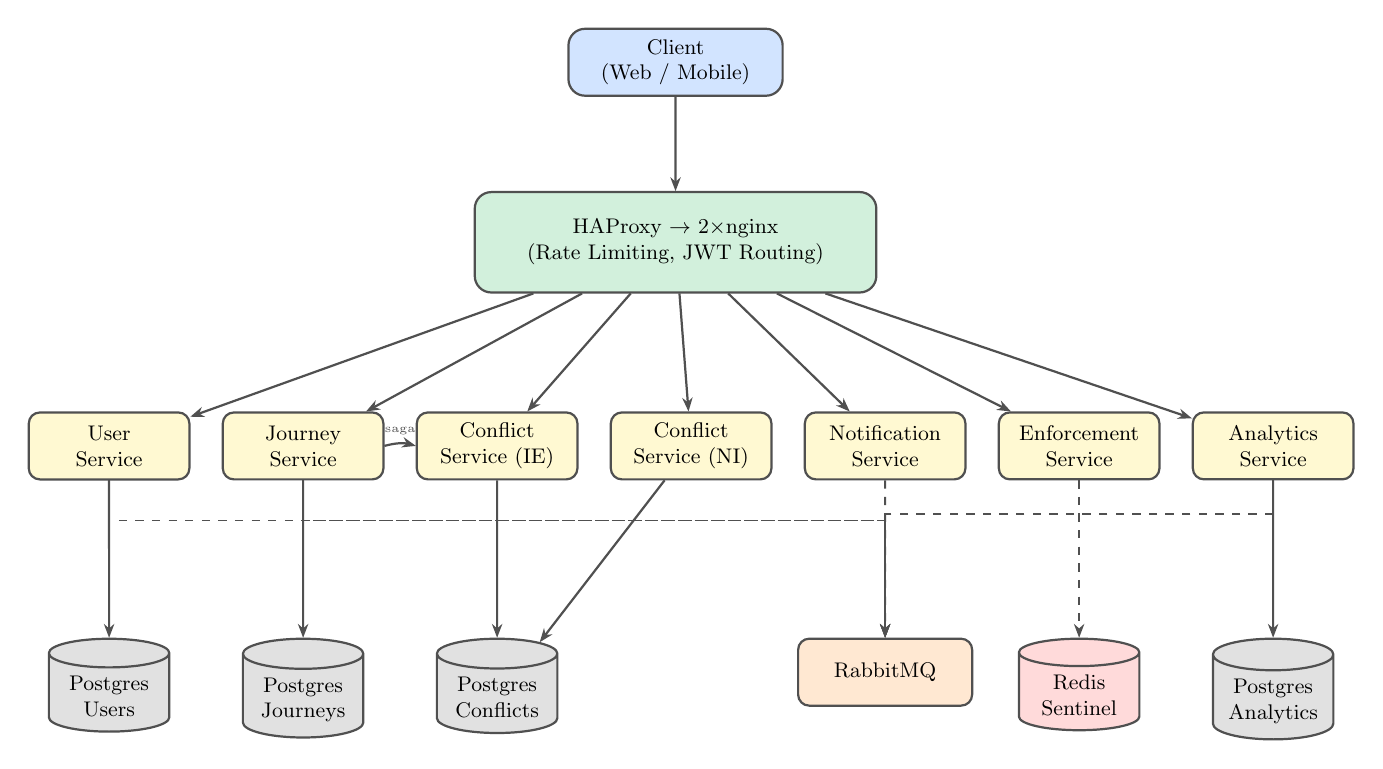
\begin{tikzpicture}[node distance=1.2cm and 0.6cm, scale=0.85, every node/.style={scale=0.85}]
  % Client
  \node[client] (client) {Client\\(Web / Mobile)};

  % Gateway
  \node[gateway, below=1.2cm of client] (gw) {HAProxy $\to$ 2$\times$nginx\\(Rate Limiting, JWT Routing)};
  \draw[arr] (client) -- (gw);

  % Services row
  \node[service, below left=1.5cm and 3.6cm of gw]  (user) {User\\Service};
  \node[service, right=0.4cm of user]   (journey) {Journey\\Service};
  \node[service, right=0.4cm of journey] (conflict) {Conflict\\Service (IE)};
  \node[service, right=0.4cm of conflict] (conflictni) {Conflict\\Service (NI)};
  \node[service, right=0.4cm of conflictni]  (notif) {Notification\\Service};
  \node[service, right=0.4cm of notif]  (enforce) {Enforcement\\Service};
  \node[service, right=0.4cm of enforce]  (analytics) {Analytics\\Service};

  % Gateway to services
  \draw[arr] (gw) -- (user);
  \draw[arr] (gw) -- (journey);
  \draw[arr] (gw) -- (conflict);
  \draw[arr] (gw) -- (conflictni);
  \draw[arr] (gw) -- (notif);
  \draw[arr] (gw) -- (enforce);
  \draw[arr] (gw) -- (analytics);

  % Infrastructure row
  \node[database, below=2cm of user]     (pguser) {Postgres\\Users};
  \node[database, below=2cm of journey]  (pgjny)  {Postgres\\Journeys};
  \node[database, below=2cm of conflict] (pgconf) {Postgres\\Conflicts};
  \node[broker, below=2cm of notif]      (rabbit) {RabbitMQ};
  \node[cache, below=2cm of enforce]     (redis)  {Redis\\Sentinel};
  \node[database, below=2cm of analytics] (pganl) {Postgres\\Analytics};

  % Service to infra
  \draw[arr] (user)      -- (pguser);
  \draw[arr] (journey)   -- (pgjny);
  \draw[arr] (conflict)  -- (pgconf);
  \draw[arr] (conflictni) -- (pgconf);
  \draw[arr] (analytics) -- (pganl);

  % All services connect to Redis and RabbitMQ (dashed)
  \draw[darr] (user.south)      -- ++(0,-0.6) -| (rabbit);
  \draw[darr] (journey.south)   -- ++(0,-0.6) -| (rabbit);
  \draw[darr] (notif)           -- (rabbit);
  \draw[darr] (enforce.south)   -- ++(0,-0.5) -| (redis);
  \draw[darr] (analytics.south) -- ++(0,-0.5) -| (rabbit);

  % Journey to Conflict (sync)
  \draw[arr, bend left=15] (journey.east) to node[above, font=\tiny]{saga} (conflict.west);

\end{tikzpicture}
\caption{High-level system architecture. Solid arrows indicate primary data flow; dashed arrows indicate event bus and cache connections.}
\end{figure}

\subsection{Technology Stack}

\begin{table}[H]
\centering\small
\begin{tabularx}{\textwidth}{l l X}
  \toprule
  \textbf{Component} & \textbf{Technology} & \textbf{Notes} \\
  \midrule
  User, Journey, Enforcement Services & Python 3.12, FastAPI & Async I/O with Uvicorn \\
  Conflict, Notification, Analytics   & Go 1.23              & chi router, pgx driver \\
  Message Broker       & RabbitMQ 3.13        & Topic exchange, dead-letter queues \\
  Cache                & Redis 7.0            & Sentinel HA (3 sentinels, quorum=2) \\
  Databases            & PostgreSQL 16        & 4 primary + 4 replicas (WAL streaming) \\
  Load Balancer        & HAProxy 2.8          & Fronts 2 nginx API gateway instances \\
  API Gateway          & nginx 1.25           & Rate limiting, JWT-based routing \\
  Containerisation     & Docker, Compose 3.8  & 26 containers (full), 12 (slim) \\
  \bottomrule
\end{tabularx}
\end{table}

\subsection{Deployment Topology}

The full deployment comprises 26 Docker containers on a single Docker Compose network (\texttt{journey-net}):
\begin{itemize}[nosep]
  \item 6 application services (7 containers: conflict service runs in 2 regions)
  \item 8 PostgreSQL containers (4 primary + 4 replicas)
  \item 3 Redis containers (1 primary, 1 replica, 3 sentinels --- 5 containers total)
  \item 1 RabbitMQ container
  \item 3 gateway containers (1 HAProxy + 2 nginx)
  \item 1 frontend container
\end{itemize}

A slim configuration (\texttt{docker-compose.slim.yml}) reduces this to 12 containers by disabling replicas and sentinels, suitable for development and low-memory environments.

\subsection{Individual Service Designs}

Each team member's most significant service is described below.

\subsubsection{Journey Service (Tanmay Ghosh)}

The Journey Service is the saga orchestrator and the most complex service. On receiving a booking request, it:
\begin{enumerate}[nosep]
  \item Validates the request and checks the idempotency key.
  \item Creates a \texttt{PENDING} journey and deducts driver points in a single database transaction using \texttt{SELECT FOR UPDATE} on the points ledger.
  \item Invokes the Conflict Service through a circuit breaker. For multi-region routes, it executes a two-phase hold/commit across regional conflict services.
  \item On success, updates the journey to \texttt{CONFIRMED} and writes an outbox event in the same transaction. On failure, marks it \texttt{REJECTED} and refunds points.
  \item A background publisher drains the outbox to RabbitMQ every 2 seconds.
\end{enumerate}

Key design decisions: the transactional outbox guarantees that events are never lost even if RabbitMQ is down; the circuit breaker prevents cascading failures when the conflict service is unreachable.

\subsubsection{Conflict Service (Sneha Meto)}

The Conflict Service models Irish roads as geographic grid cells (0.01\textdegree{} resolution, approximately 1~km). Each cell has a configurable maximum capacity per time slot. The core algorithm:
\begin{enumerate}[nosep]
  \item Receives a booking request with origin, destination, and departure time.
  \item Computes all grid cells along the route using waypoint interpolation.
  \item For each cell, calculates the estimated arrival time based on distance from origin.
  \item Within a \texttt{SERIALIZABLE} transaction with \texttt{SELECT FOR UPDATE}, checks that no cell exceeds capacity for the requested time window.
  \item If all cells pass, inserts booking records atomically. Otherwise, returns a conflict response.
\end{enumerate}

For cross-border journeys, the service supports a two-phase protocol: \texttt{hold} reserves capacity tentatively, \texttt{commit} finalises, and \texttt{rollback} releases the hold.

\subsubsection{User Service (Parth Deshmukh)}

The User Service provides stateless JWT-based authentication. It routes read queries to a Postgres replica and writes to the primary. On registration, it publishes a \texttt{user.registered} event to RabbitMQ so that Analytics can track sign-ups. Vehicles are associated with user accounts and validated for uniqueness on the registration plate.

\subsubsection{Notification Service (Aditya Kumar Singh)}

The Notification Service consumes events from RabbitMQ and pushes them to connected clients via WebSocket. An in-memory registry maps user IDs to WebSocket connections. Notifications are also persisted in Redis (7-day TTL, max 50 per user) for clients that reconnect. Consumer deduplication via Redis \texttt{SETNX} on message IDs ensures that redelivered messages do not generate duplicate notifications.

\subsubsection{Enforcement Service (Saurabh Deshmukh)}

The Enforcement Service provides low-latency verification for roadside agents. It uses a Redis-first lookup pattern: active journeys are cached by vehicle plate and user ID (populated by consuming \texttt{journey.confirmed} events). On cache miss, it falls back to the Journey Service REST API. Licence-to-user-ID mappings are cached for 24 hours. When the Journey Service is partitioned, the service returns cached data with an \texttt{X-Cache-Stale} header.

\subsubsection{Analytics Service (Sai Eeshwar Divaakar)}

The Analytics Service performs dual-write logging to both PostgreSQL and Redis. A background goroutine runs hourly rollups, aggregating event counts into an \texttt{hourly\_stats} table. It also monitors Postgres streaming replication lag across all service databases and exposes an aggregated health endpoint that probes all six services.

% ═════════════════════════════════════════════════════════════════════════════
\section{Implementation}
% ═════════════════════════════════════════════════════════════════════════════

\subsection{Journey Booking Flow}

Figure~\ref{fig:booking-flow} shows the sequence of operations for a successful journey booking.

\begin{figure}[H]
\centering
\begin{tikzpicture}[
  actor/.style={rectangle, draw, minimum width=2cm, minimum height=0.7cm, font=\small},
  note/.style={font=\tiny, align=left},
  arr/.style={-{Stealth[length=4pt]}, font=\tiny},
  node distance=0.4cm
]
  % Actors
  \node[actor] (client) at (0,0) {Client};
  \node[actor] (jny)    at (3.5,0) {Journey Svc};
  \node[actor] (conf)   at (7,0) {Conflict Svc};
  \node[actor] (rmq)    at (10.5,0) {RabbitMQ};

  % Lifelines
  \draw[dashed, gray] (client.south) -- ++(0,-8);
  \draw[dashed, gray] (jny.south)    -- ++(0,-8);
  \draw[dashed, gray] (conf.south)   -- ++(0,-8);
  \draw[dashed, gray] (rmq.south)    -- ++(0,-8);

  % Messages
  \draw[arr] (0,-1) -- node[above]{POST /api/journeys/} (3.5,-1);
  \draw[arr] (3.5,-2) -- node[above]{POST /api/conflicts/check} (7,-2);
  \node[note, right] at (7.2,-2.5) {SERIALIZABLE tx};
  \draw[arr] (7,-3) -- node[above]{APPROVED} (3.5,-3);
  \node[note, right] at (3.7,-3.5) {UPDATE journey=CONFIRMED};
  \node[note, right] at (3.7,-4) {INSERT outbox\_event};
  \node[note, right] at (3.7,-4.5) {(same transaction)};
  \draw[arr] (3.5,-5.2) -- node[above]{200 OK (confirmed)} (0,-5.2);
  \draw[arr, dashed] (3.5,-6.2) -- node[above]{publish event} (10.5,-6.2);
  \node[note, right] at (10.7,-6.7) {fan-out to 4 queues};
\end{tikzpicture}
\caption{Sequence diagram for journey booking.}
\label{fig:booking-flow}
\end{figure}

\subsection{Failure Detection: Partition Manager}

The partition manager is a shared component (\texttt{shared/partition.py}) used by the Journey and Enforcement services to detect network partitions. It implements a state machine:

\begin{figure}[H]
\centering
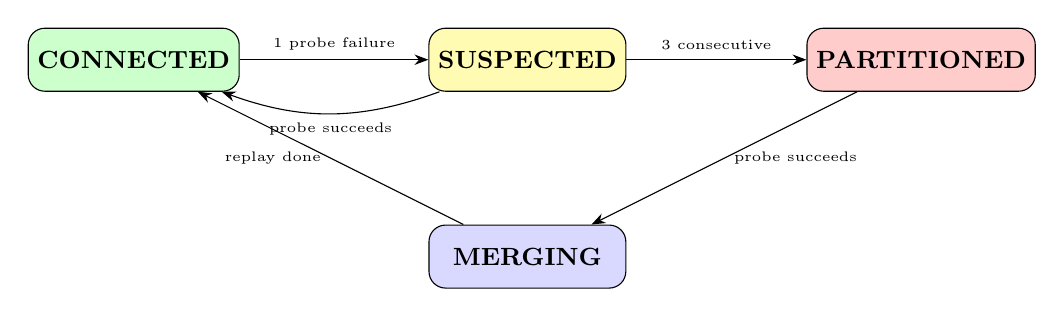
\begin{tikzpicture}[
  state/.style={rectangle, rounded corners=6pt, draw, minimum width=2.5cm, minimum height=0.8cm, font=\small\bfseries},
  arr/.style={-{Stealth[length=5pt]}, font=\tiny},
]
  \node[state, fill=green!20] (conn) at (0,0) {CONNECTED};
  \node[state, fill=yellow!30] (susp) at (5,0) {SUSPECTED};
  \node[state, fill=red!20] (part) at (10,0) {PARTITIONED};
  \node[state, fill=blue!15] (merg) at (5,-2.5) {MERGING};

  \draw[arr] (conn) -- node[above]{1 probe failure} (susp);
  \draw[arr] (susp) -- node[above]{3 consecutive} (part);
  \draw[arr] (susp) to[bend left=20] node[below]{probe succeeds} (conn);
  \draw[arr] (part) -- node[right]{probe succeeds} (merg);
  \draw[arr] (merg) -- node[left]{replay done} (conn);
\end{tikzpicture}
\caption{Partition manager state machine. Probes run every 5 seconds against each dependency (Postgres, Redis, RabbitMQ, Conflict Service).}
\end{figure}

Each dependency (Postgres, Redis, RabbitMQ, Conflict Service) is monitored independently. When a dependency enters the PARTITIONED state, the service:
\begin{itemize}[nosep]
  \item Adds \texttt{X-Partition-Status: true} to HTTP responses.
  \item Queues write operations locally (max 1000 entries).
  \item On merge, replays queued operations with last-writer-wins conflict resolution.
\end{itemize}

\subsection{Circuit Breaker}

The circuit breaker (\texttt{shared/circuit\_breaker.py}) wraps calls from the Journey Service to the Conflict Service:

\begin{itemize}[nosep]
  \item \textbf{CLOSED}: Requests pass through normally. Failures are counted.
  \item \textbf{OPEN}: After 3 failures, all requests fail immediately with \texttt{CircuitBreakerOpenError} for 30 seconds.
  \item \textbf{HALF-OPEN}: One probe request is allowed. On success, the circuit closes. On failure, it re-opens.
\end{itemize}

This prevents the Journey Service from saturating its thread pool with requests to an unresponsive Conflict Service.

\subsection{Transactional Outbox}

The Journey Service guarantees that events are published to RabbitMQ even when the broker is temporarily unavailable:

\begin{enumerate}[nosep]
  \item When a journey is confirmed or rejected, an event row is inserted into the \texttt{journey\_events} outbox table \emph{in the same database transaction} as the journey state change.
  \item A background thread polls the outbox every 2 seconds, publishes pending events to RabbitMQ, and marks them as published only after broker acknowledgement.
  \item If RabbitMQ is down, events accumulate in the outbox and are drained when connectivity resumes.
\end{enumerate}

\subsection{Consumer Deduplication}

All four asynchronous consumers (Notification, Conflict, Analytics, Enforcement) implement idempotent message handling:
\begin{itemize}[nosep]
  \item On receiving a message, the consumer computes a deduplication key from the message ID (or SHA-256 of the body if no ID is present).
  \item A Redis \texttt{SETNX} with 24-hour TTL is used to check if the message has already been processed.
  \item If already processed, the message is acknowledged and skipped.
  \item This ensures at-least-once delivery does not produce duplicate side effects.
\end{itemize}

\subsection{Multi-Region Saga (Two-Phase Protocol)}

For journeys crossing regional boundaries (e.g.\ Dublin to Belfast), the Journey Service orchestrates a two-phase saga:

\begin{enumerate}[nosep]
  \item \textbf{Phase 1 --- Hold}: The Journey Service sends \texttt{POST /api/conflicts/hold} to each regional Conflict Service. Each service tentatively reserves capacity and returns a hold ID.
  \item \textbf{Phase 2 --- Commit}: If all regions return successful holds, the Journey Service sends \texttt{POST /api/conflicts/commit/\{hold\_id\}} to each region.
  \item \textbf{Rollback}: If any region fails in Phase 1, all previously successful holds are rolled back via \texttt{POST /api/conflicts/rollback/\{hold\_id\}}.
\end{enumerate}

\textbf{Limitation}: If a network failure occurs during Phase 2 (after some commits succeed but before all complete), the system may enter a partial-commit state. This is logged but not automatically resolved.

\subsection{Grid-Cell Capacity Algorithm}

The Conflict Service models road capacity using a geographic grid:

\begin{enumerate}[nosep]
  \item Roads are represented as sequences of waypoints (latitude, longitude).
  \item The grid resolution is 0.01\textdegree{} ($\approx$ 1~km).
  \item For a booking request, the algorithm walks the route in 1~km steps, computing the grid cell for each point and interpolating the arrival time based on distance from the origin.
  \item For each cell and time window, the algorithm checks the current booking count against the cell's maximum capacity using \texttt{SELECT FOR UPDATE} within a \texttt{SERIALIZABLE} transaction.
  \item If any cell is at capacity, the entire booking is rejected atomically.
\end{enumerate}

\subsection{Dead-Letter Queue Handling}

All consumers are configured with a dead-letter exchange (\texttt{journey\_events\_dlx}). Messages that are explicitly rejected (\texttt{nack} without requeue) or exceed retry limits are routed to the \texttt{dead\_letter\_queue} with a 24-hour TTL. Administrative endpoints (e.g.\ \texttt{/admin/recovery/drain-outbox}) allow manual replay of failed messages.

% ═════════════════════════════════════════════════════════════════════════════
\section{Testing}
% ═════════════════════════════════════════════════════════════════════════════

\subsection{Test Plan}

Testing was conducted at three levels:

\begin{enumerate}
  \item \textbf{Unit testing}: Individual service logic (Go test files, Python unit tests) covering input validation, grid-cell computation, and circuit breaker state transitions.
  \item \textbf{Integration testing}: Automated end-to-end demo script (\texttt{scripts/demo\_local.py}) that exercises the full system on Docker.
  \item \textbf{Fault injection}: Manual and scripted fault scenarios using simulation endpoints and Docker container manipulation.
\end{enumerate}

\subsection{End-to-End Demo Script}

The automated demo (\texttt{scripts/demo\_local.py}) verifies 11 scenarios sequentially:

\begin{table}[H]
\centering\small
\caption{End-to-end test scenarios}
\begin{tabularx}{\textwidth}{C{0.6cm} L{4cm} X}
  \toprule
  \textbf{\#} & \textbf{Scenario} & \textbf{Verification} \\
  \midrule
  1 & Service health        & All 6 services return healthy status \\
  2 & User registration     & Driver and agent accounts created successfully \\
  3 & Vehicle registration  & Vehicle linked to driver account \\
  4 & Journey booking       & Journey confirmed; conflict check passed \\
  5 & Conflict detection    & Second overlapping booking rejected \\
  6 & Async event fan-out   & Notification, analytics, and enforcement cache all updated \\
  7 & Enforcement lookup    & Vehicle verified from Redis cache \\
  8 & Journey cancellation  & Capacity released; events propagated \\
  9 & Outbox recovery       & RabbitMQ killed mid-booking; events delivered after restart \\
  10 & Circuit breaker      & Conflict service killed; 3 bookings fail fast \\
  11 & Partition detection  & Network partition simulated; staleness headers present \\
  \bottomrule
\end{tabularx}
\end{table}

\subsection{Fault Injection Tests}

The following fault scenarios were tested manually:

\begin{itemize}[nosep]
  \item \textbf{RabbitMQ failure}: \texttt{docker stop rabbitmq}, book a journey, \texttt{docker start rabbitmq} --- verified that outbox drained and all consumers received the event.
  \item \textbf{Conflict Service failure}: \texttt{docker stop conflict-service-ie} --- verified circuit breaker opens after 3 failures and closes on recovery.
  \item \textbf{Redis Sentinel failover}: Killed Redis primary --- verified sentinel promoted replica and services reconnected automatically.
  \item \textbf{Postgres replica failure}: Stopped a replica container --- verified services fell back to primary reads.
  \item \textbf{Simulated delay}: \texttt{POST /api/simulate/delay} with 5-second latency --- verified timeout handling.
\end{itemize}

\subsection{Load Testing}

A load test script (\texttt{scripts/load\_test.py}) was used to verify system behaviour under concurrent booking requests, testing the serialisable isolation level's ability to prevent double-booking under contention.

\subsection{Test Results}

All end-to-end demo scenarios pass on the Docker slim stack. The full stack (with replicas and sentinels) has been verified for failover scenarios. The RabbitMQ 3-node cluster configuration is present but Erlang distribution proved unreliable on a single Docker host; the single-node configuration demonstrates all messaging principles correctly.

% ═════════════════════════════════════════════════════════════════════════════
\section{Allocation of Work}
% ═════════════════════════════════════════════════════════════════════════════

\begin{table}[H]
\centering
\caption{Work allocation across team members}
\begin{tabularx}{\textwidth}{l l X}
  \toprule
  \textbf{Member} & \textbf{Primary Service} & \textbf{Additional Contributions} \\
  \midrule
  Parth Deshmukh & User Service & JWT authentication, primary/replica DB routing, user.registered event publishing \\
  \addlinespace
  Tanmay Ghosh & Journey Service & Saga orchestration, transactional outbox, circuit breaker, partition detection, idempotency, lifecycle scheduler \\
  \addlinespace
  Sneha Meto & Conflict Service & Grid-cell algorithm, SERIALIZABLE transactions, two-phase hold/commit, route definitions, fault simulation endpoints \\
  \addlinespace
  Aditya Kumar Singh & Notification Service & WebSocket push, Redis notification history, consumer deduplication, dead-letter queue \\
  \addlinespace
  Saurabh Deshmukh & Enforcement Service & Redis-first cache, licence lookup, partition-aware staleness headers, event-driven cache population \\
  \addlinespace
  Sai Eeshwar Divaakar & Analytics Service & Dual-write logging, hourly rollup, replica lag monitoring, aggregated health endpoint \\
  \bottomrule
\end{tabularx}
\end{table}

\textbf{Shared infrastructure} (Docker Compose, API gateway, Redis Sentinel, Postgres replication, RabbitMQ configuration, shared Python libraries for partition detection and circuit breaking) was developed collaboratively.

% ═════════════════════════════════════════════════════════════════════════════
\section{Summary}
% ═════════════════════════════════════════════════════════════════════════════

We have designed and implemented a distributed journey booking system comprising six microservices that demonstrates over 20 distributed systems principles in a realistic, end-to-end scenario. The key achievements are:

\begin{itemize}
  \item \textbf{Fault-tolerant booking pipeline}: The saga pattern with a transactional outbox ensures that no booking event is lost, even under message broker failures. Consumer deduplication guarantees exactly-once processing semantics.

  \item \textbf{Atomic conflict detection}: Road capacity is enforced via geographic grid cells with \texttt{SERIALIZABLE} database transactions, preventing double-booking under concurrent load.

  \item \textbf{Multi-region coordination}: Cross-border journeys are handled by a two-phase hold/commit protocol across regional conflict services, demonstrating distributed transaction coordination.

  \item \textbf{Comprehensive failure handling}: Circuit breakers prevent cascading failures, partition detection enables graceful degradation, Redis Sentinel provides cache high availability, and Postgres streaming replication ensures data durability.

  \item \textbf{Real-time communication}: WebSocket notifications provide immediate feedback to drivers, while the event bus ensures all services stay eventually consistent.

  \item \textbf{Observable and testable}: Every service exposes health endpoints, partition status is tracked per-dependency, replica lag is monitored, and an automated demo script validates all critical paths including fault scenarios.
\end{itemize}

\textbf{Known limitations}: Compensating transactions for saga rollback are not implemented (the system rejects rather than retries on failure). The WebSocket connection registry is in-memory only. The enforcement cache is cold on startup. Distributed tracing with span visualisation (Jaeger/Zipkin) is not integrated. These represent areas for future work.

The system has been verified end-to-end on Docker Compose, demonstrating correct operation under normal conditions and graceful degradation under the fault scenarios described in this report.

\end{document}
